\chapter{Teorie - Možnosti určení času}
\label{4-teorie-urceni-casu}
Existuje mnoho možností, jak synchronizovat čas. Mezi nejběžnější patří synchronizace pomocí internetu, rádiového signálu nebo GNSS přijímače.

\section{Internet}
Na internetu jsou dostupné zdroje poskytující informace o~aktuálním koordinovaném světovém čase UTC. Hlavní výhodou synchronizace času pomocí internetu je její snadná dostupnost. Tato metoda je dostupná celosvětově na všech místech s~připojením k~internetu. Nevýhodou je, že může být přesnost synchronizace času ovlivněna latencí internetového připojení. Nejčastěji se lze setkat s~\zk{API} a \zk{NTP} servery.

\subsection{API}
\zkratka{API} je rozhraní, které slouží pro předávání dat mezi softwarovými aplikacemi.
\zk{API} může být použito k~získání času z~webové služby. Například, World Time API slouží pro získání aktuálního času a poskytuje čas pro konkrétní časová pásma ve tvaru Unixového času, nebo ve tvaru podle ISO8601. Data jsou poskytována ve formátu prostého textu nebo jako JSON \cite{worldtimeapi}.

\subsection{NTP}
\zkratka{NTP} servery jsou nejběžněji využívaným zdrojem pro synchronizaci času přes internet. \zk{NTP} je navržený tak, aby na něj neměla velký vliv proměnlivá latence internetového připojení. K~posílání informací slouží v~\zk{NTP} serverech takzvané packety, které obsahují vždy menší množství dat. K~omezení vlivu latence internetového připojení jsou využívány sofistikované algoritmy, díky nimž se přesnost synchronizace času pohybuje do 10 ms \cite{timetools}. Příkladem NTP serveru je Google Public NTP a NTP Pool \cite{ntppool}.
%https://home.zcu.cz/~poupa/pccas.html
% 50ms je sntp
%klasické ntp je lepší : https://timetoolsltd.com/ntp/ntp-timing-accuracy/

\section{Rádiový signál}
Existují vysílače, které vysílají informace o~čase pomocí radiových vln. Tyto signály jsou obvykle velmi přesné, ale jejich příjem může být ovlivněn atmosférickými podmínkami nebo rušením signálu. Příkladem těchto vysílačů jsou WWVB v~USA, MSF ve Velké Británii a DCF77 v~Německu. V~minulosti existoval v~ČR vysílač OMA 50, který od roku 1995 není v~provozu \cite{vyvoj_hw_poupa}.% seznam vysílačů: https://en.wikipedia.org/wiki/Radio_clock

\subsection{DCF77}
Vzhledem k~omezenému dosahu rádiového signálu má na území ČR smysl uvažovat o~využití pouze signálu DCF77. Vysílač DCF77 vysílá čas vycházející z~měření cesiových atomových hodin Fyzikálně-technického institutu v~Braunschweigu (PTB). Tento vysílač vysílá dlouhovlnné rádiové vlny na kmitočtu 77,5 kHz. Výkon vysílače je 50kW. Vysílač vysílá nepřetržitě od roku 1970 a odstaven je jen velmi výjimečně z~důvodů údržby. Teoretický dosah vysílače je uváděn až 2000 km, což však platí jen za ideálních podmínek. Dosah vysílače i za méně příznivých podmínek je udáván 1100~km, což stále pokrývá celé území České republiky.\cite{ptb_dcf77} Název DCF77 vychází z~označení:
\begin{description}[leftmargin=!,labelwidth=\widthof{\bfseries D --}]
    \item[\textbf{D} --] Deutschland (Německo)
    \item[\textbf{C} --] Označení pásma dlouhých vln
    \item[\textbf{F} --] Frankfurtský region
    \item[\textbf{77} --] Vysílací frekvence (77,5 kHz)
\end{description}

\textbf{Časový kód signálu DCF77:}
Každou minutu vysílač vysílá informaci o~\text{minutě}, hodině, dni v~týdnu, měsíci a roku pomocí amplitudové modulace. Tato \text{informace} platí vždy pro následující minutu \cite{fel_dcf77}. Dále je signál modulován pomocí pseudo\-náhodné fázové modulace, která slouží pro přenos pseudonáhodného šumu, který lze využít pro přesnější určení času \cite{vyvoj_hw_poupa} \cite{ptb_2012}.

\begin{figure}[H]
	\centering
	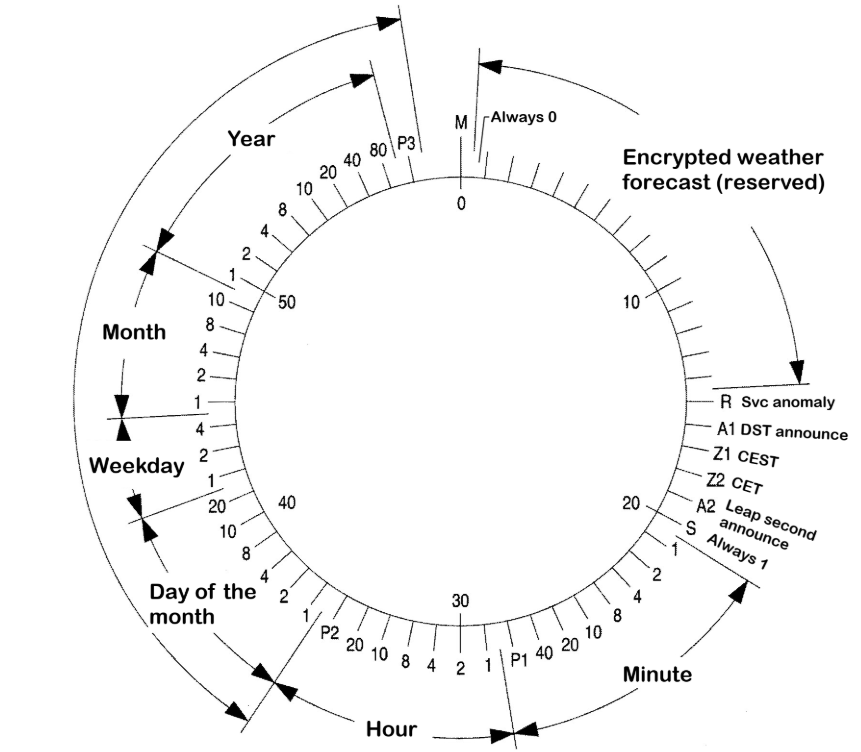
\includegraphics[width=8.4cm]{images/komponenty/schema_DCF77_signalu_lepsi.png}
	\caption{Schéma signálu DCF 77 \cite{fel_dcf77}}
\end{figure}

\textbf{Rušení signálu DCF77:}
Signál DCF77 se šíří ohybem po povrchu Země a odrazem od ionosféry. Odrazy od ionosféry jsou přes den slabé, a proto je signál během dne slabší. Signál DCF77 je rušen z~několika zdrojů. Jedním zdrojem rušení je atmosférický šum způsobený činností ionosféry a může dosahovat velikosti až 80~dB. Atmosférický šum je proměnlivý. Dále může být signál rušen průmyslovou činností, například vlivem vysokonapěťového vedení \cite{vyvoj_hw_andel} \cite{hopf_dcf77}.

\section{GNSS}
Pro určení času lze využít \zkratka{GNSS} jako je GPS, GLONASS nebo Galileo. Družice těchto systémů vysílají časové informace spolu s~navigačními daty. Na satelitech těchto systémů jsou obvykle cesiové atomové hodiny a záložní rubidiové atomové hodiny, které poskytují velmi přesný zdroj času. Signál z těchto družic jsou schopny přijímat GNSS přijímače. Signál je ovšem z~důvodu tranzitní doby opožděn. Pokud přijímač přijímá v~jednu epochu signál alespoň ze čtyř družic, je schopen spočítat opravu hodin přijímače a tím získat svůj přesný čas. Tento čas poskytují GNSS přijímače prostřednictvím NMEA zprávy.

Je potřeba si uvědomit, že například GPS družice pracují v~GPS čase, který je odlišný od času UTC. Součástí NMEA zprávy \$GNZDA je však už čas přepočítaný do UTC \cite{ublox}. Tato metoda poskytuje velmi přesný čas a je dostupná kdekoliv na Zemi, ale vyžaduje přímý výhled na oblohu pro příjem signálů od alespoň čtyř satelitů, aby bylo možné spočítat i opravu hodin přijímače.

